\subsubsection{Descrizione generale}
Questo servizio svolge l'importante funzione di fornire delle API\G{} RESTful al Frontend\G{} della piattaforma.
Queste permettono di svolgere le azioni richieste dall'utente, soprattutto l'ottenimento di dati dal database.
Il servizio viene eseguito in ambiente container, gestito da AWS\G{} Fargate.

\subsubsection{Diagramma delle classi}
\begin{figure}[H]
    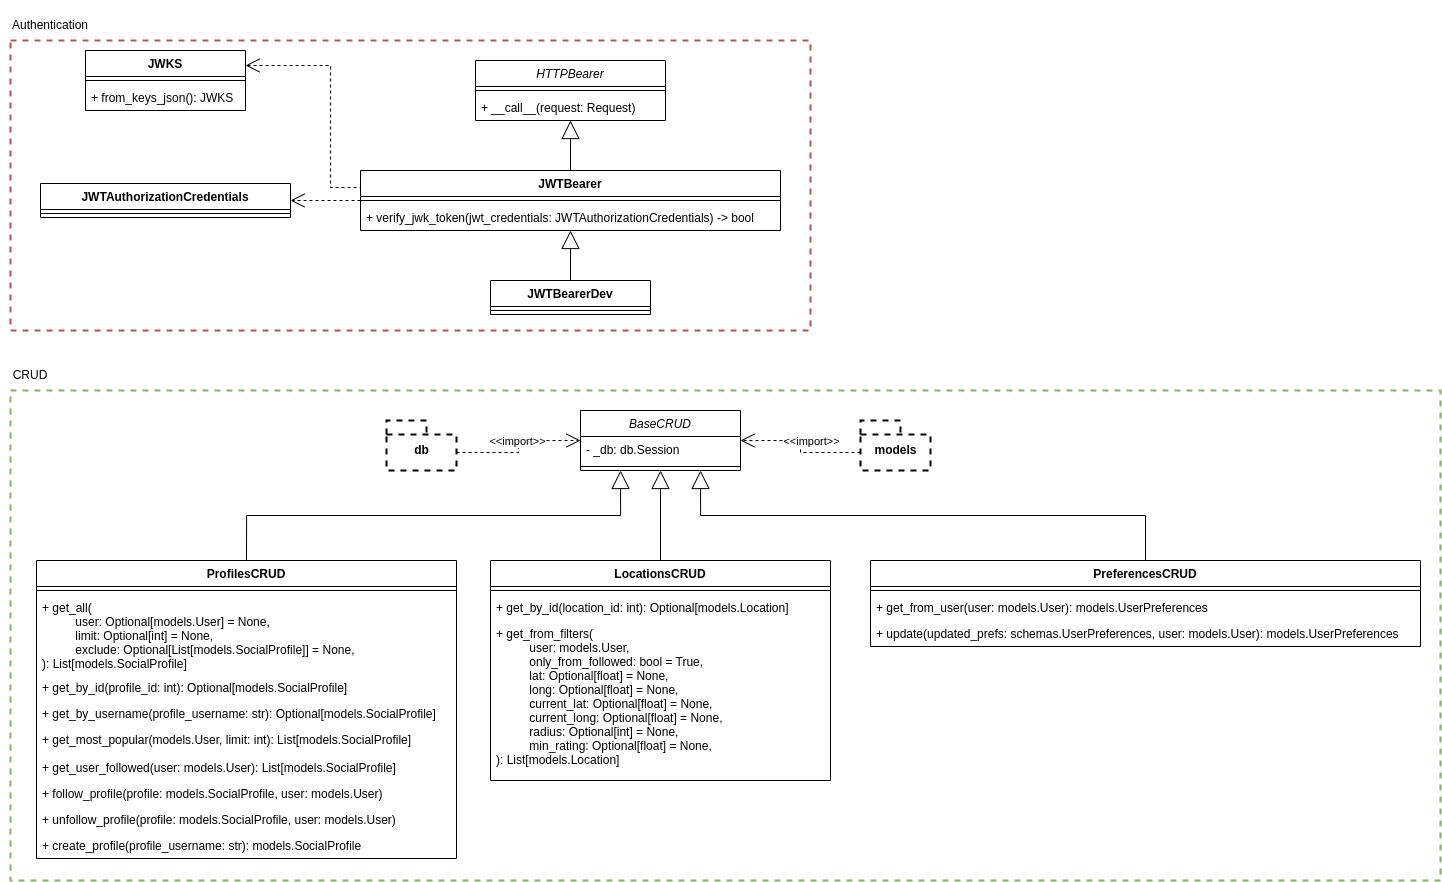
\includegraphics[width=16cm]{sezioni/images/cd_api.png}
    \centering
    \caption{API Service - Diagramma delle classi}
\end{figure}

\subsubsection{Implementazione}
Per l'implementazione del servizio è stato scelto FastAPI, un framework\G{} Python\G{} per lo sviluppo di API\G.\\
Essendo Python\G{} un linguaggio multiparadigma, ed il framework\G{} non increntrato sul paradigma ad oggetti, non sono state definite gerarchie di classi particolarmente complesse.
Degne di nota sono le classi derivanti da \verb|BaseCRUD|, che si occupano di gestire operazioni
di lettura e scrittura dal database, quindi buona parte della \textit{business logic}.\\
La gestione degli \textit{endpoint} delle API\G{} avviene tramite decoratori a funzioni.
I dati delle richieste, sia essi di percorso o nel \textit{body} della richiesta stessa, vengono passati alla funzione come dei normali parametri grazie al funzionamento interno di FastAPI.

\begin{lstlisting}[language=Python, caption=Esempio di gestione di un \textit{endpoint}]
@router.get(
    '/locations/{location_id}',
    response_model=schemas.Location,
    response_model_exclude_unset=True,
)
def get_location(
    location_id: int,
    locations: LocationsCRUD = Depends(get_locations_crud),
):
    location = locations.get_by_id(location_id)
    if not location:
        raise HTTPException(status_code=HTTP_404_NOT_FOUND, detail='Location not found')
    return location
\end{lstlisting}

\paragraph{Documentazione automatica}\aCapo
Le API\G{} vengono documentate automaticamente dal framework\G, seguendo lo standard OpenAPI.

\subsubsection{Autenticazione}
L'autenticazione degli utenti avviene tramite JWT\G{}. Il token è memorizzato nell'header HTTP \verb|Authentication|,
e viene impostato dopo il login dall'interfaccia di Cognito\G. La verifica della validità avviene nella classe \verb|JWTBearer|.
Tale verifica avviene dopo ogni chiamata ad endpoint che necessitano di autenticazione.
\begin{figure}[H]
    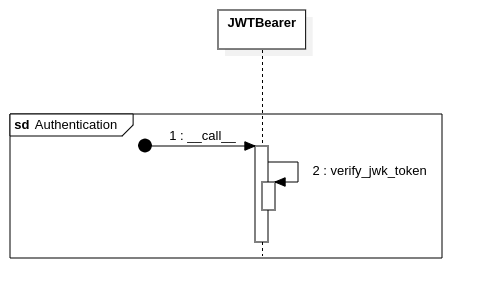
\includegraphics[width=8cm]{sezioni/images/sd_api_auth.png}
    \centering
    \caption{Autenticazione - Diagramma di sequenza}
\end{figure}
